\documentclass[10pt,a4paper]{scrartcl}
\setkomafont{disposition}{\normalfont\bfseries}
\usepackage[utf8]{inputenc}
\usepackage[french]{babel}
\usepackage[T1]{fontenc}
\usepackage{amsmath}
\usepackage{amsthm}
\usepackage{amsfonts}
\usepackage{amssymb}
\usepackage{graphicx}
\usepackage{mathrsfs}
\usepackage{url}
\usepackage{color}
\usepackage{hyperref}
\usepackage{cleveref}
\usepackage{listings}
\definecolor{mygreen}{RGB}{28,172,0} % color values Red, Green, Blue
\definecolor{mylilas}{RGB}{170,55,241}
\lstset{
language=R,
basicstyle=\scriptsize\ttfamily,
commentstyle=\ttfamily\color{green},
numbers=left,
numberstyle=\ttfamily\color{black}\footnotesize,
stepnumber=1,
numbersep=5pt,
backgroundcolor=\color{white},
showspaces=false,
showstringspaces=false,
showtabs=false,
frame=single,
tabsize=2,
captionpos=b,
breaklines=true,
breakatwhitespace=false,
keywordstyle=\color{blue},
stringstyle=\color{magenta},
literate=
  {á}{{\'a}}1 {é}{{\'e}}1 {í}{{\'i}}1 {ó}{{\'o}}1 {ú}{{\'u}}1
  {Á}{{\'A}}1 {É}{{\'E}}1 {Í}{{\'I}}1 {Ó}{{\'O}}1 {Ú}{{\'U}}1
  {à}{{\`a}}1 {è}{{\`e}}1 {ì}{{\`i}}1 {ò}{{\`o}}1 {ù}{{\`u}}1
  {À}{{\`A}}1 {È}{{\'E}}1 {Ì}{{\`I}}1 {Ò}{{\`O}}1 {Ù}{{\`U}}1
  {ä}{{\"a}}1 {ë}{{\"e}}1 {ï}{{\"i}}1 {ö}{{\"o}}1 {ü}{{\"u}}1
  {Ä}{{\"A}}1 {Ë}{{\"E}}1 {Ï}{{\"I}}1 {Ö}{{\"O}}1 {Ü}{{\"U}}1
  {â}{{\^a}}1 {ê}{{\^e}}1 {î}{{\^i}}1 {ô}{{\^o}}1 {û}{{\^u}}1
  {Â}{{\^A}}1 {Ê}{{\^E}}1 {Î}{{\^I}}1 {Ô}{{\^O}}1 {Û}{{\^U}}1
  {œ}{{\oe}}1 {Œ}{{\OE}}1 {æ}{{\ae}}1 {Æ}{{\AE}}1 {ß}{{\ss}}1
  {ű}{{\H{u}}}1 {Ű}{{\H{U}}}1 {ő}{{\H{o}}}1 {Ő}{{\H{O}}}1
  {ç}{{\c c}}1 {Ç}{{\c C}}1 {ø}{{\o}}1 {å}{{\r a}}1 {Å}{{\r A}}1
  {€}{{\EUR}}1 {£}{{\pounds}}1
}

\lstset{language=Matlab,%
%basicstyle=\color{red},
breaklines=true,%
morekeywords={matlab2tikz},
keywordstyle=\color{blue},%
morekeywords=[2]{1}, keywordstyle=[2]{\color{black}},
identifierstyle=\color{black},%
stringstyle=\color{mylilas},
commentstyle=\color{mygreen},%
showstringspaces=false,%without this there will be a symbol in the places where there is a space
numbers=left,%
numberstyle={\tiny \color{black}},% size of the numbers
numbersep=9pt, % this defines how far the numbers are from the text
emph=[1]{for,end,break},emphstyle=[1]\color{red}, %some words to emphasise
%emph=[2]{word1,word2}, emphstyle=[2]{style},    
}
\lstset{literate=
{á}{{\'a}}1 {é}{{\'e}}1 {í}{{\'i}}1 {ó}{{\'o}}1 {ú}{{\'u}}1
{Á}{{\'A}}1 {É}{{\'E}}1 {Í}{{\'I}}1 {Ó}{{\'O}}1 {Ú}{{\'U}}1
{à}{{\`a}}1 {è}{{\`e}}1 {ì}{{\`i}}1 {ò}{{\`o}}1 {ù}{{\`u}}1
{À}{{\`A}}1 {È}{{\'E}}1 {Ì}{{\`I}}1 {Ò}{{\`O}}1 {Ù}{{\`U}}1
{ä}{{\"a}}1 {ë}{{\"e}}1 {ï}{{\"i}}1 {ö}{{\"o}}1 {ü}{{\"u}}1
{Ä}{{\"A}}1 {Ë}{{\"E}}1 {Ï}{{\"I}}1 {Ö}{{\"O}}1 {Ü}{{\"U}}1
{â}{{\^a}}1 {ê}{{\^e}}1 {î}{{\^i}}1 {ô}{{\^o}}1 {û}{{\^u}}1
{Â}{{\^A}}1 {Ê}{{\^E}}1 {Î}{{\^I}}1 {Ô}{{\^O}}1 {Û}{{\^U}}1
{œ}{{\oe}}1 {Œ}{{\OE}}1 {æ}{{\ae}}1 {Æ}{{\AE}}1 {ß}{{\ss}}1
{ű}{{\H{u}}}1 {Ű}{{\H{U}}}1 {ő}{{\H{o}}}1 {Ő}{{\H{O}}}1
{ç}{{\c c}}1 {Ç}{{\c C}}1 {ø}{{\o}}1 {å}{{\r a}}1 {Å}{{\r A}}1
{€}{{\euro}}1 {£}{{\pounds}}1 {«}{{\guillemotleft}}1
{»}{{\guillemotright}}1 {ñ}{{\~n}}1 {Ñ}{{\~N}}1 {¿}{{?`}}1
}
\usepackage[french,onelanguage,ruled,lined,linesnumbered]{algorithm2e}
\SetKw{And}{et}
\SetKw{From}{allant de}
\author{\textsc{BOUCETTA I.} \& \textsc{TRAN Q.N.H.} \& \textsc{WARTELLE A.}}
\title{Rapport de projet OS10}
\subtitle{Etude de l'algorithme GRASP pour le problème d'ordonnancement FJSSP-nfa}
\date{\today}

\begin{document}
\maketitle
\renewcommand{\contentsname}{Sommaire}
\tableofcontents
\clearpage

\begin{abstract}
Ce travail a pour objectif d'étudier l'article de 2010 de Rajkumar, Muthukannan \& Asokan, P \& Vamsikrishna, V.
portant sur un algorithme de recherche locale randomisée : \emph{Greedy Randomized Adaptive Search Procedure} (GRASP),
dans le cadre d'un problème de job shop : le \emph{Flexible Job Shop Scheduling Problem with non fixed-availability constraints}
(FJSSP-nfa) \cite{GRASP}. 
Cette extension du problème du job shop permet de prendre en compte deux aspects importants de la production :
\begin{enumerate}
\item la flexibilité des machines pour effectuer des opérations, c'est-à-dire qu'une opération n'aura pas une machine
prédéfinie à l'avance pour son exécution. On aura en effet le choix entre plusieurs machines avec différents temps
d'exécution associés. Cette diversité des temps d'exécution est en général lié à la performance et à l'adéquation de chaque machine
pour exécuter une tâche
\item la prise en compte de tâches de maintenance à effectuer dans des fenêtres de temps données (indisponibilité non fixe). En effet
les machines ont besoin d'être entretenues afin d'éviter (si possible) des pannes ou des défaillances. Durant une
tâche de maintenance, une machine et indisponible est ne peut pas traiter d'opération, ce qui impacte fortement
les performances d'un choix d'affectation d'opérations et d'ordonnancement de celles-ci.
\end{enumerate}
Avec la prise en compte de la flexibilité des machines, le FJSSP-nfa permet de travailler sur de nouveaux
critères portant sur la charge de travail, c'est à dire sur le temps d'utilisation de chaque machine qui
n'est plus fixé comme dans le cas d'un job shop classique (CJSSP). Ainsi le FJSSP-nfa est un problème multi-critère portant
sur la charge de travail totale et maximal des machines et sur le makespan de l'ordonnancement (temps
de complétion maximale).

Le problème de job shop classique étant déjà NP-difficile, le FJSSP-nfa l'est aussi.
De plus, avec les difficultés rajoutées par la flexibilité des machines et la maintenance,
une approche de résolution par méthode exacte est presque inenvisageable\footnote{d'après \cite{GA1},
les méthodes exactes par graphes disjonctifs sont actuellement limités à 20 jobs et 10 machines pour
le FJSSP (sans maintenance)}. Ainsi ce sont des heuristiques comme l'algorithme de recherche locale GRASP (\cite{GRASP}) 
et des méta-heuristiques comme les algorithmes génétiques(\cite{GA1},\cite{GA2}) qui rencontrent le plus de succès pour ce type de problème car elle permettent d'avoir de bons résultats multi-critères  en un temps raisonnable.

\end{abstract}

\section{Définitions : FJSSP-nfa et GRASP}

Avec la notation de Graham, le problème d'ordonnancement FJSSP-nfa peut s'écrire sous la forme : 
\[J_{m}|flexibility,nfa|W_{tot},W_{max},C_{max}\]
Plus précisément, on souhaite minimiser une combinaison linéaire de $W_{tot}$ (charge totale
d'occupation des machines),$W_{max}$ (charge maximale
d'occupation des machines) et $C_{max}$ :
$W_1*W_{tot}+W_2*W_{max}+W_3*C_{max}$ avec $W_1+W_2+W_3=1$ et $W_1$,$W_2$,$W_3$ des paramètres
donnés en fonction des préférences d'objectif.

En reprenant les notations de l'article \cite{GRASP}, on a $n$ jobs d'incice $i$
avec $n_{i}$ opérations d'indice $k$ pour chaque job $i$ (notées $O_{ik}$), $m$ machine d'indice $j$, $L_{j}$ tâches de maintenance d'indice $l$ pour chaque machine $j$ (notées $PM_{jl}$). Chaque opération
peut être affectées sur un ensemble $A_{ik}$ de machines avec différentes durées $t_{ikj}$
d'exécution. Les tâches de maintenance ont des durées $p_{jl}$ d'exécution et doivent se terminées
sur des fenêtres de temps $[t^{E}_{jl},t^{L}_{jl}]$ ($E$ pour "Early" et $L$ pour "Late"). \\

L'algorithme GRASP est un algorithme de recherche locale randomisée avec une approche hiérarchique
pour résoudre le FJSSP-nfa, c'est-à-dire qu'il va d'abord résoudre le problème d'affectation
des opérations $O_{ik}$ aux machines de $A_{ik}$ ($\forall i,k$) puis le problème d'ordonnancement
des opérations $O_{ik}$ affectées et des tâches de maintenance  $PM_{jl}$ sur chaque machine\footnote{L'approche
hiérarchique s'oppose à l'approche intrinsèque où les deux problèmes sont résolus conjointement, cette approche
est plus difficile mais peut donner de meilleurs résultats notamment avec les algorithmes génétiques}.
Comme le montre les algorithmes \ref{algo:routing} et \ref{algo:scheduling} (voir aussi \cite{GRASP}), GRASP va construire
une solution en ajoutant itérativement les opérations \footnote{les tâches de maintenance sont ajoutées par des
détections de conflit avec l'ordonnancement d'uen opération et lorsque toutes les opérations ont pu être ordonnancées}
 (pour l'affectation et l'ordonnancement) qui sont choisies de manière
aléatoire dans une liste RCL de candidats restreinte. 

La RCL est un voisinage de l'opération qui fait augmenter le moins
la valeur de la fonction objective ($W_{tot}$ pour l'algorithme 1 et $C_{max}$ pour l'algorithme 2). La RCL est triée par valeur croissante des augmentations de la valeur objective
afin de pondérer la probabilité de choisir chaque candidat (opération à affecter) en fonction de son rang $r$
avec la fonction $r \rightarrow 1/r$.

La taille de la RCL est paramétrée par une valeur $\alpha \in [0,1]$ qui
va permettre de fixer la valeur maximale d'augmentation de la fonction objective (pour être
acceptée dans la liste) par $OFV_{min}+\alpha*(OFV_{max}-OFV_{min})$ avec $OFV_{min}$ et $OFV_{max}$
les valeurs minimales et maximales (respectivement) de la fonction objective après l'ajout de la prochaine opération.

Finalement, pour chaque itération principale de l'algorithme, on sélectionne aléatoirement (avec un générateur (pseudo-)aléatoire de loi uniforme)
une valeur  $\alpha \in [0,1]$ qui sera utilisée pour construire une solution
complète au problème de FJSSP-nfa. On obtient ainsi une ensemble de solutions
où chacune indique les affectations $x_{ikj} \in \{0,1\}$ (ou $x_{ik} \in \{0,1...,j\}$ dans
notre algorithme) et les temps de complétions $c_{ik}$ et $y_{jl}$ des opérations $O_{ik}$
et des tâches de maintenances $PM_{jl}$ respectivement. On sélectionne enfin la solution
qui minimise la fonction objective $W_1*W_{tot}+W_2*W_{max}+W_3*C_{max}$.

\begin{algorithm}
  \caption{Assigner les opérations aux machines (\emph{routing})}
  \label{algo:routing}
  \tcp{Initialisation}
  $t$ le nombre de solutions\;
  $A = \{\alpha_1, \alpha_2,..., \alpha_t\}$ l'ensemble des valeurs $\alpha$ discrètes aléatoires telle que $0 \leq \alpha_i \leq 1 \, \forall i = \overline{1,t}$\;
  $S = \{s_1, s_2,..., s_t\}$ l'ensemble des solutions à construire\;
  \tcp{Assignment}
  \ForEach{$\alpha_i \in A$}{
    $\sigma$ l'ensemble des opérations non assignées\;
    $s_i$ la solution à construire\;
    $s_i \leftarrow \emptyset$\;
    \While{$\sigma \neq \emptyset$}{
      \tcp{Le processing time $t_o$ dépend de la machine de traitement et correspond à l'augmentation de $W_{tot}$ (de $s_i$) par l'affectation d'une opération}
      Chercher $O_{Max}$ l'opération dont le processing time est le plus long\;
      Chercher $O_{min}$ l'opréation dont le processing time est le plus court\;
      $Range \leftarrow t_{O_{Max}} - t_{O_{min}}$\;
      $Width \leftarrow Range * \alpha_i$\;
      Construire RCL l'ensemble des opérations non assignées $o \in \sigma$ telle que $t_{O_{min}} \leq t_o \leq t_{O_{min}} + Width$\;
      Ordonner RCL dans l'ordre croissant de processing time\;
      Pondérer les éléments de RCL par la fonction $\frac{1}{r}$ où $r$ est l'ordre de l'élément\;
      Choisir de manière aléatoire un élément $o^*$ de RCL en tenant compte des poids ci-dessus (la probabilité de choisir une opération o est $\frac{poids_o}{poids_{total}}$)\;
      $s_i \leftarrow s_i \cup o^*$\;
      $\sigma \leftarrow \sigma \backslash o^*$\;
    }
    Calculer la charge totale de $s_i$\;
  }
\end{algorithm}

\begin{algorithm}
  \caption{Ordonner les opérations et les maintenances sur les machines (\emph{scheduling})}
  \label{algo:scheduling}
  \tcp{Initialisation}
  $t$ le nombre de solutions (fixé à l'algorithme \eqref{algo:routing}) \;
  $A = \{\alpha_1, \alpha_2,..., \alpha_t\}$ l'ensemble des valeurs $\alpha$ discrètes aléatoires telle que $0 \leq \alpha_i \leq 1 \, \forall i = \overline{1,t}$ (pas forcément identique à l'algorithme \eqref{algo:routing})\;
  $S = \{s_1, s_2,..., s_t\}$ l'ensemble des solutions à construire\;
  \tcp{Ordonnancement}
  \ForEach{$\alpha_i \in A$}{
    $\sigma$ l'ensemble des opérations non ordonnées\;
    $s_i$ la solution à ordonner\;
    $s_i \leftarrow \emptyset$\;
    \While{$\sigma \neq \emptyset$}{
      \tcp{Le processing time dépend de machine de traitement}
      Chercher $o_{Max}$ l'opération qui augmente le plus $C_{max}$ (de $s_{i}$); et $o_{min}$ l'opération qui augmente le moins $C_{max}$ en tenant compte les maintenances dont les temps de complétion doivent se situer dans les intervalles donnés $\left[t_{jl}^E, t_{jl}^L\right]$ \;
      $Range \leftarrow C_{max}^{o_{Max}} -C_{max}^{o_{min}}$\;
      $Width \leftarrow 1 + Range * \alpha_i$\;
      Construire RCL l'ensemble des opérations non assignées $o \in \sigma$ telle que $C_{max}^{o_{min}} \leq C_{max}^{o} \leq C_{max}^{o_{min}} + Width$\;
      Ordonner RCL dans l'ordre croissant des $C_{max}$\;
      Pondérer les éléments de RCL par la fonction $\frac{1}{r}$ où $r$ est l'ordre de l'élément\;
      Choisir de manière aléatoire un élément $o^*$ de RCL en tenant compte des poids ci-dessus (la probabilité de choisir une opération o est $\frac{poids_o}{poids_{total}}$\;
      Ordonner $o^*$ en tenant compte la date de disponibilité la plus tôt et les maintenances\;
      $\sigma \leftarrow \sigma \backslash o^*$\;
    }
    Ordonner les maintenances sans collision à la suite opérations ordonnancées\;
    Calculer le makespan ($C_{max}$) de $s_i$\;
  }
\end{algorithm}

\section{Résultats et comparaisons}
%
%\begin{figure}[!ht]
%    \centering
%    \includegraphics[width=0.8\linewidth]{img/PPI1.png}
%    \caption{Chemin de l'algorithme PPI}
%    \label{PPI1}
%\end{figure}
\subsection{Spécification de l'ordinateur}
Nous tournons le code sur un ordinateur portable de processeur Intel(R) Core(TM) i7-7700HQ CPU\@2.8GHz (8 CPUs), 8 Go de RAM. Le programme est compilé par Visual Studio Code 2017. Le générateur choisi est \texttt{MersenneTwister.h} (v1.0, 15/05/2003).

\subsection{Résultats et comparaisons avec ceux de l'article}
Nous réalisons $1000$ solutions (itérations) séquentiellement parmi lesquelles nous choissions les meilleurs corresponsdant au triplet voulu.
\begin{table}[!h]
  \centering
  \begin{tabular}{|c|c|c|}
    \hline
    Critères & Valeurs de l'article & Nos valeurs \\
    \hline
    $W_t$ & 103 & 103 \\
    $W_{max}$ & 16 & 15 \\
    $C_{max}$ & 18 & 18 \\
    $F(0.5;0.3;0.2)$ & 59.9 & 59.9 \\
    $F(0.5;0.2;0.3)$ & 60.1 & 60.1 \\
    \hline
  \end{tabular}
  \caption{Résultat pour problème $8 \times 8$}
\end{table}

\begin{table}[!h]
  \centering
  \begin{tabular}{|c|c|c|}
    \hline
    Critères & Valeurs de l'article & Nos valeurs \\
    \hline
    $W_t$ & 60 & 60 \\
    $W_{max}$ & 7 & 8 \\
    $C_{max}$ & 9 & 12 \\
    $F(0.5;0.3;0.2)$ & 33.9 & 35.4 \\
    $F(0.5;0.2;0.3)$ & 34.1 & 35.6 \\
    \hline
  \end{tabular}
  \caption{Résultat pour problème $10 \times 10$}
\end{table}

\begin{table}[!h]
  \centering
  \begin{tabular}{|c|c|c|}
    \hline
    Critères & Valeurs de l'article & Nos valeurs \\
    \hline
    $W_t$ & 107 & 98 \\
    $W_{max}$ & 13 & 14 \\
    $C_{max}$ & 16 & 19 \\
    $F(0.5;0.3;0.2)$ & 60.3 & 57.2 \\
    $F(0.5;0.2;0.3)$ & 60.9 & 57.8 \\
    \hline
  \end{tabular}
  \caption{Résultat pour problème $15 \times 10$}
\end{table}

\begin{table}[!h]
  \centering
  \begin{tabular}{|c|c|c|}
    \hline
    Critères & Valeurs de l'article & Nos valeurs \\
    \hline
    $W_t$ & 40 & 40 \\
    $W_{max}$ & 9 & 9 \\
    $C_{max}$ & 16 & 12 \\
    $F(0.5;0.3;0.2)$ & 25.9 & 25.6 \\
    $F(0.5;0.2;0.3)$ & 26.6 & 25.9 \\
    \hline
  \end{tabular}
  \caption{Résultat pour problème $4 \times 5$}
\end{table}

Nos valeurs sont très proche celles trouvées dans l'articles, particulièrement certaines sont meilleures, signifiant la reproductivité facile de l'algorithme. Son application aura peu de dépendance de l'ordinateur de planification au niveau de résultat.

D'autre part, au niveau de temps d'exécution, qui joue un rôle important de chaque algorithme, leurs déroulement ne prennent pas plus de \emph{2 seconds} (figure \eqref{tab:temps_exec}). Autrement dit, l'algorithme GRASP est efficace contre le problème de type FJSSP-nfa.

\begin{table}[!h]
  \centering
  \begin{tabular}{|c|c|c|}
    \hline
    Problème & Temps d'exécution (ms) \\
    \hline
    $4 \times 5$ & 28.6767 \\
    $8 \times 8$ & 150.71 \\
    $10 \times 10$ & 427.403 \\
    $15 \times 10$ & 1661.43 \\
    \hline
  \end{tabular}
  \caption{Temps d'exécution de chaque problème exemplaire}
  \label{tab:temps_exec}
\end{table}

Les ordonnancements finaux pour chaque problème exemplaire sont inclus dans l'annexe \eqref{annexe:visual_ordo}.

\subsection{Analyse supplémentaire : frontières de dominance de Pareto}

Afin de compléter l'analyse donnée par l'article, nous avons décidé de regarder
les frontières de dominance de Pareto sur 5 niveaux (le niveau i dominant le niveau i+1)
qui sont disponibles en annexes \ref{annexe:visual_pareto}.
Nous avons observé que, tout en ayant 1000 solutions, les premières frontières sont composées de très peu de
vecteurs de solutions (composé des trois valeurs objectives)
 avec en général seulement 2 pour la première frontière et quelques dizaines au total pour les
5 premières. De plus les solutions sont assez bien distribuées dans l'espace et on a pas trop de vecteurs objectifs (environ 2 ou 3 au maximum)
identiques.

On remarque que les objectifs à minimiser sont souvent positivement corrélés, c'est-à-dire que la diminution de l'un implique souvent la diminution d'au moins l'un des autres. Cela semble logique puisque moins de  charge de travail permettra souvent aux machines de terminer plus tôt (makespan diminué) et terminer plus tôt nécessite souvent d'avoir moins de charge.
Néanmoins l'ajout d'une recherche locale randomisée permet de découvrir des solutions souvent meilleurs et peu évidentes car elles peuvent aller à l'encontre de cette corrélation positive. 
Ainsi, l'algorithme GRASP semble être une approche adaptée pour résoudre le FJSSP-nfa en multi-objectifs.


\section{Annexes}

\subsection{Visualisation de tournées (plotJob.m)}
\lstinputlisting[language=Matlab]{src/plotJob.m}

\subsection{Visualisation de frontières de dominance de Pareto (plotFront.m)}
\lstinputlisting[language=Matlab]{src/plotFront.m}

\subsection{Visualisation des ordonnancements}
\label{annexe:visual_ordo}
\begin{figure}
  \centering
  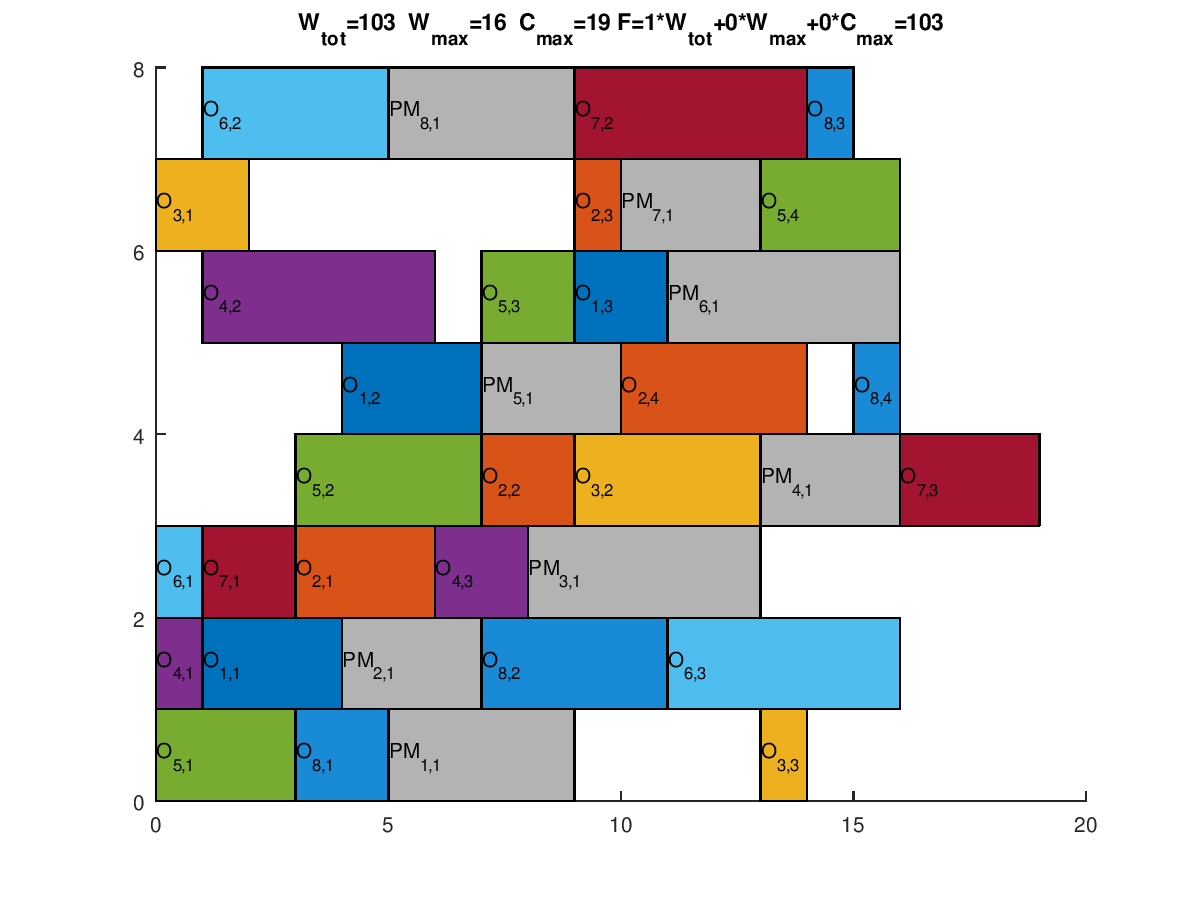
\includegraphics[width=0.8\textwidth]{img/results8x8_Wtot.png}
  \caption{$8 \times 8$ $W_{t}$ : $(W_t, W_{max}, C_{max}) = (103; 16; 19)$}
\end{figure}
\begin{figure}
  \centering
  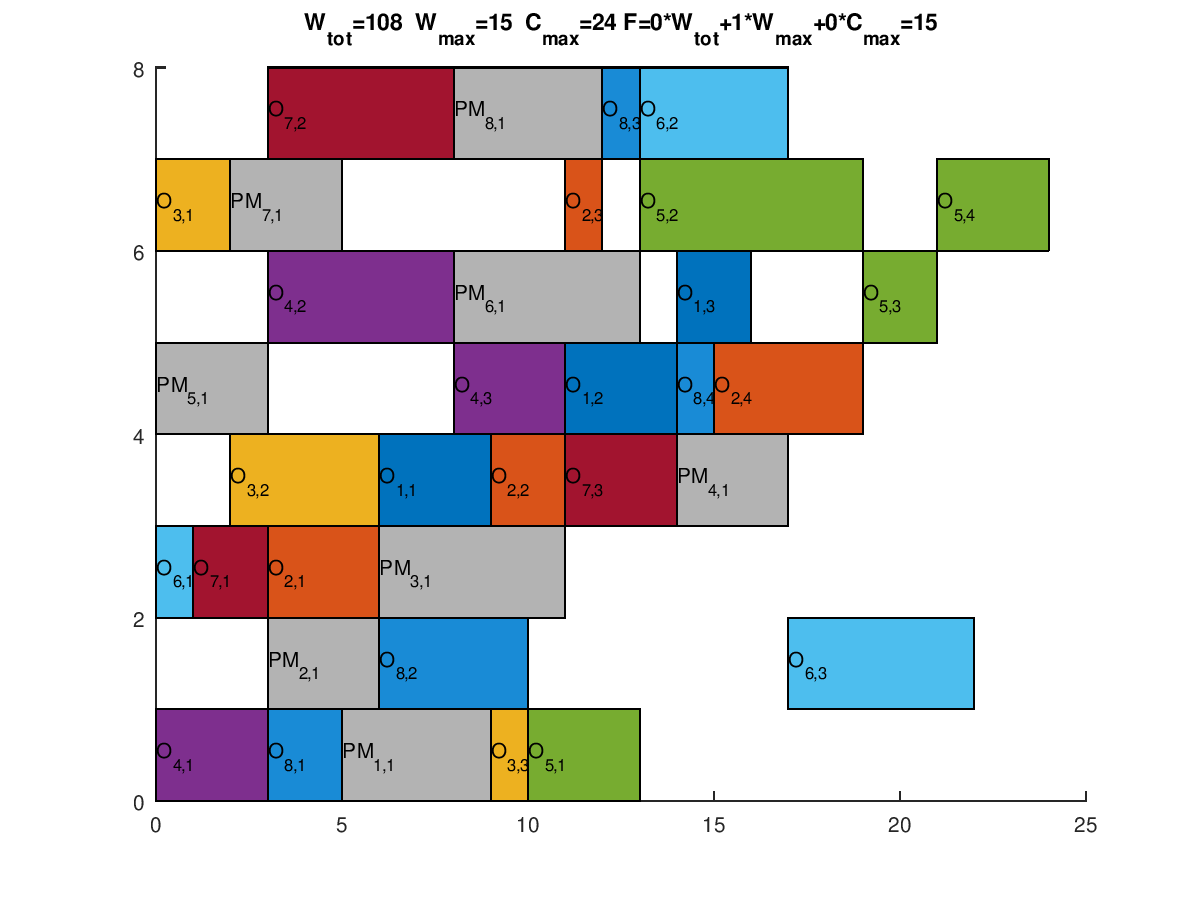
\includegraphics[width=0.8\textwidth]{img/results8x8_Wmax.png}
  \caption{$8 \times 8$ $W_{max}$ : $(W_t, W_{max}, C_{max}) = (108; 15; 24)$}
\end{figure}
\begin{figure}
  \centering
  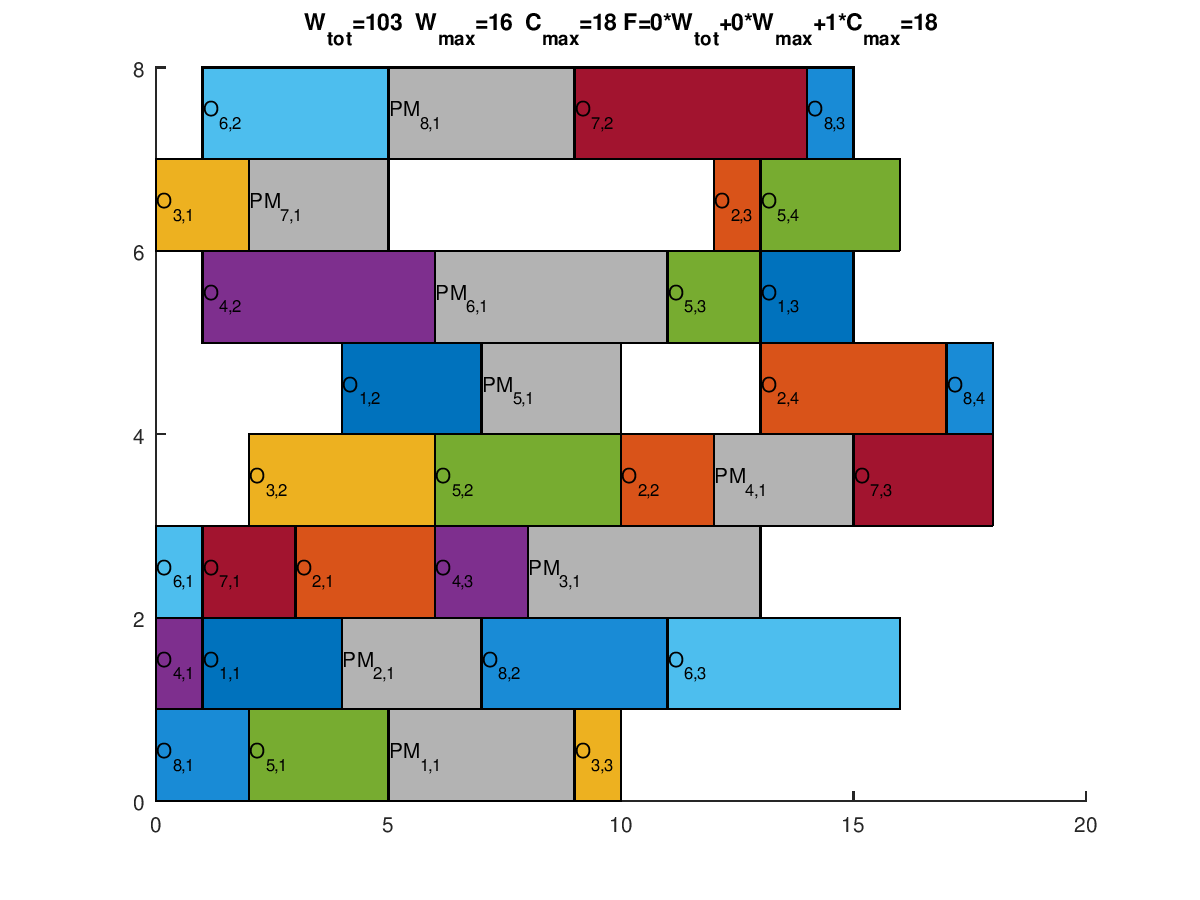
\includegraphics[width=0.8\textwidth]{img/results8x8_Cmax.png}
  \caption{$8 \times 8$ $C_{max}$ : $(W_t, W_{max}, C_{max}) = (103; 16; 18)$}
\end{figure}
\begin{figure}
  \centering
  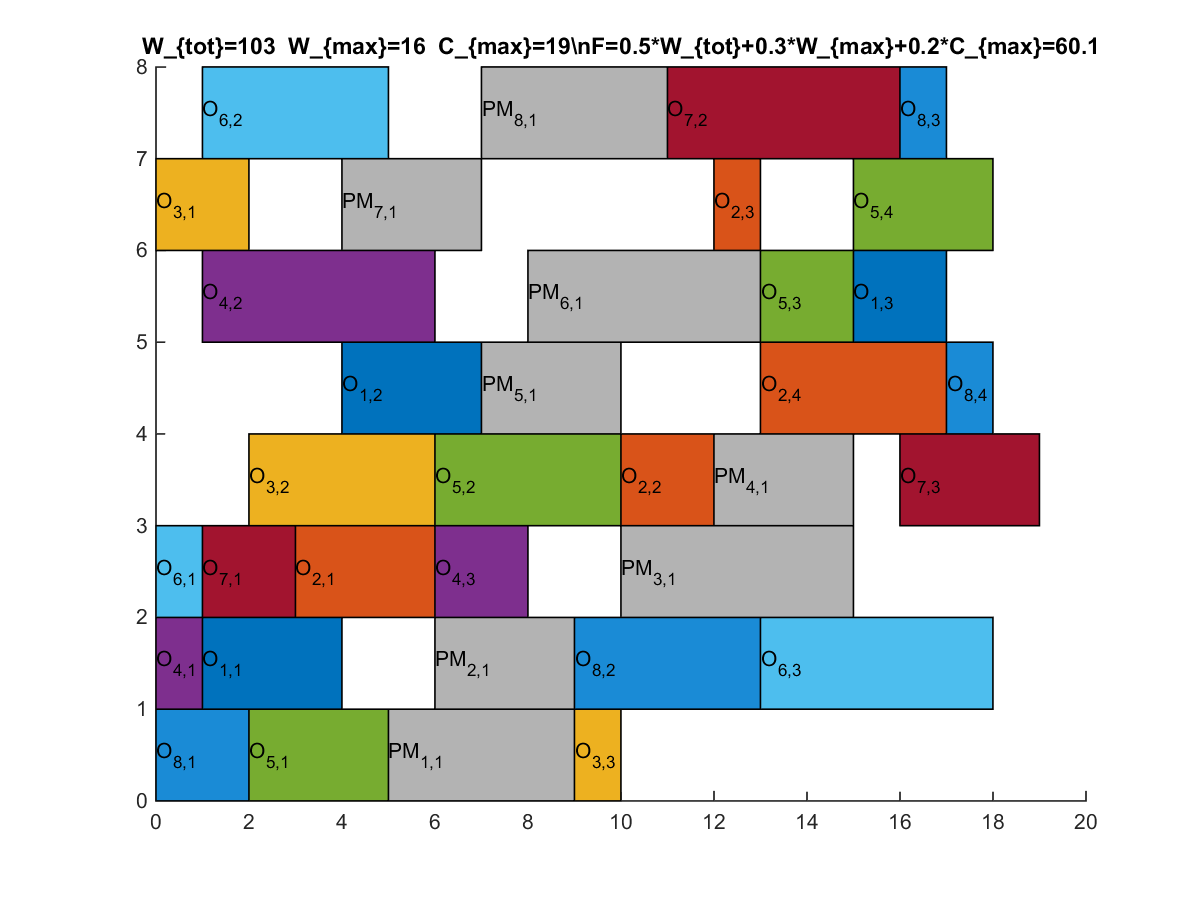
\includegraphics[width=0.8\textwidth]{img/results8x8_F050302.png}
  \caption{$8 \times 8$ $F(0.5;0.3;0.2)$ : $(W_t, W_{max}, C_{max}) = (103; 16; 18)$}
\end{figure}
\begin{figure}
  \centering
  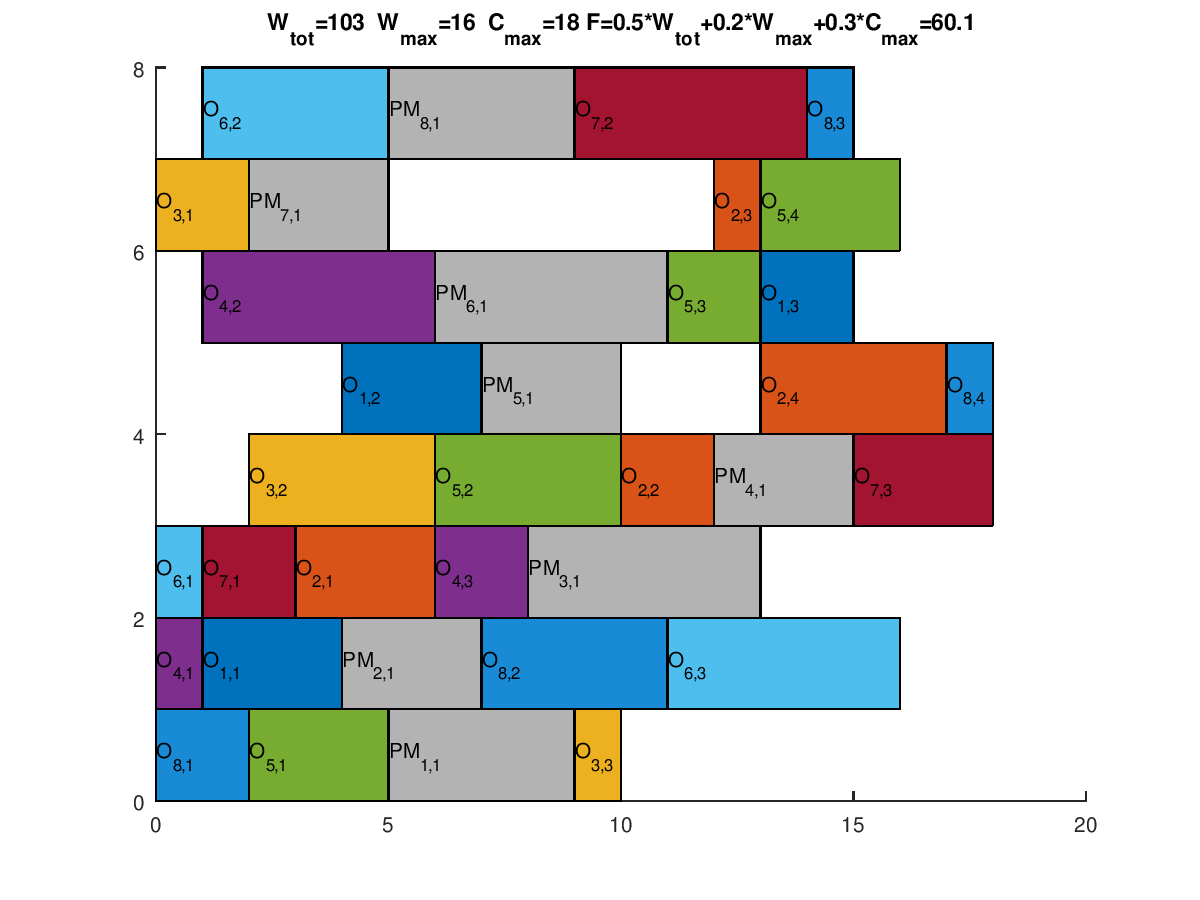
\includegraphics[width=0.8\textwidth]{img/results8x8_F050203.png}
  \caption{$8 \times 8$ $F(0.5;0.2;0.3)$ : $(W_t, W_{max}, C_{max}) = (103; 16; 18)$}
\end{figure}
\begin{figure}
  \centering
  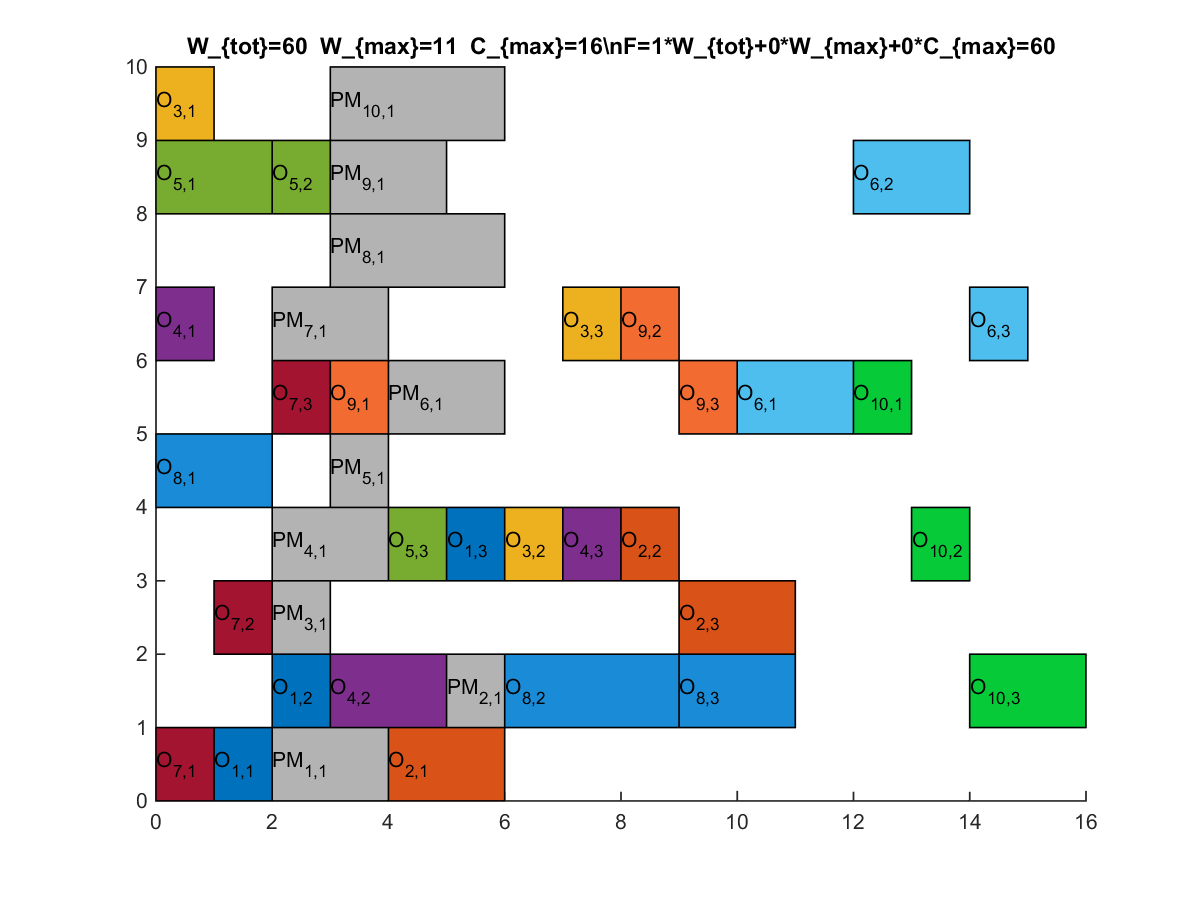
\includegraphics[width=0.8\textwidth]{img/results10x10_Wtot.png}
  \caption{$10 \times 10$ $W_{t}$ : $(W_t, W_{max}, C_{max}) = (60; 11; 15)$}
\end{figure}
\begin{figure}
  \centering
  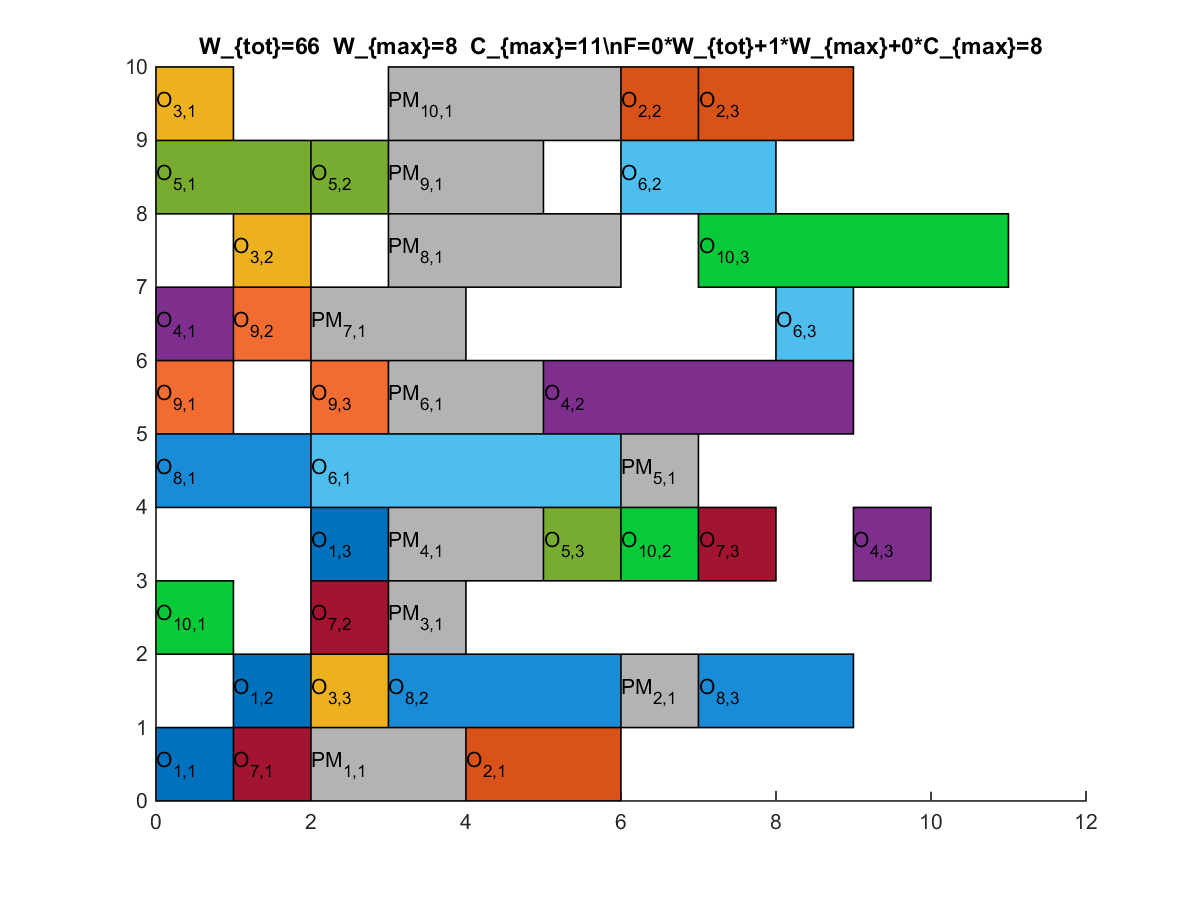
\includegraphics[width=0.8\textwidth]{img/results10x10_Wmax.png}
  \caption{$10 \times 10$ $W_{max}$ : $(W_t, W_{max}, C_{max}) = (66; 8; 13)$}
\end{figure}
\begin{figure}
  \centering
  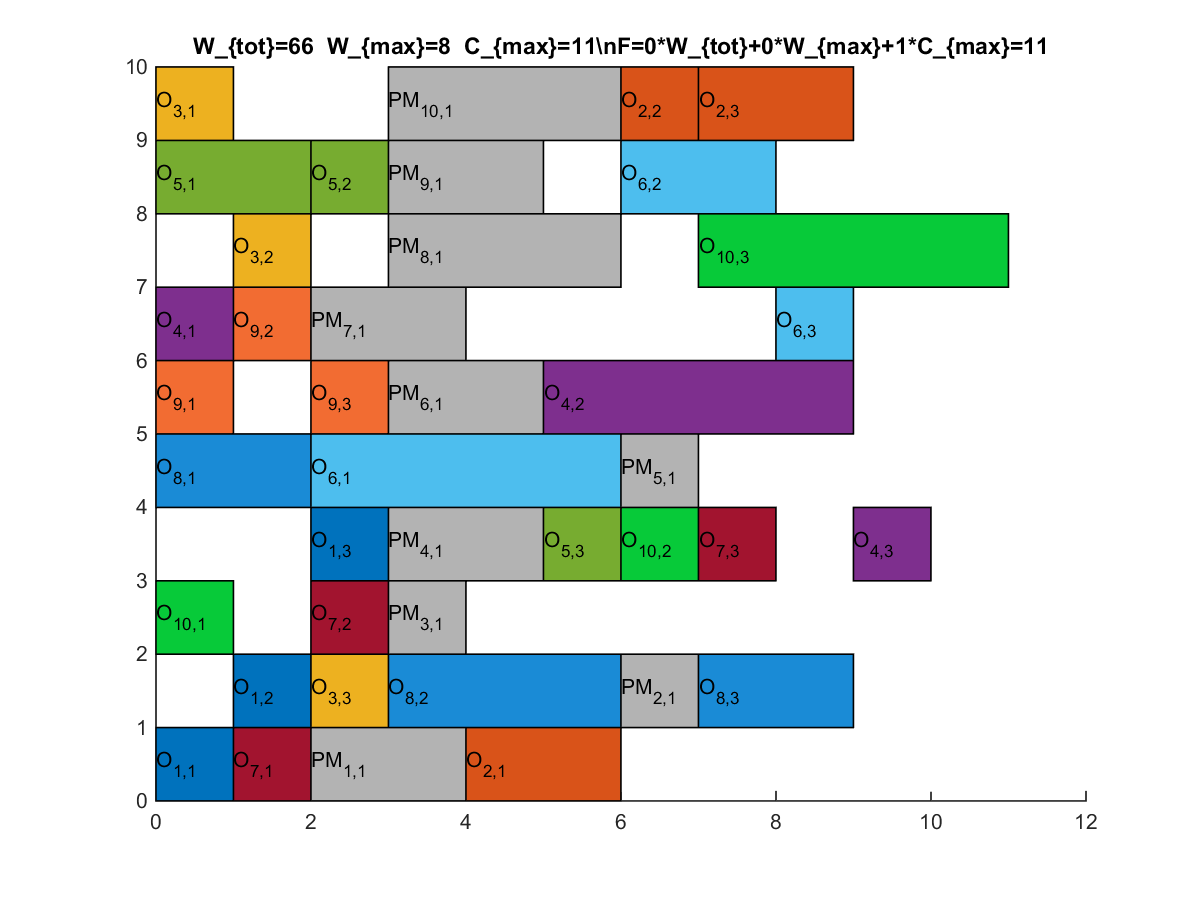
\includegraphics[width=0.8\textwidth]{img/results10x10_Cmax.png}
  \caption{$10 \times 10$ $C_{max}$ : $(W_t, W_{max}, C_{max}) = (62; 12; 12)$}
\end{figure}
\begin{figure}
  \centering
  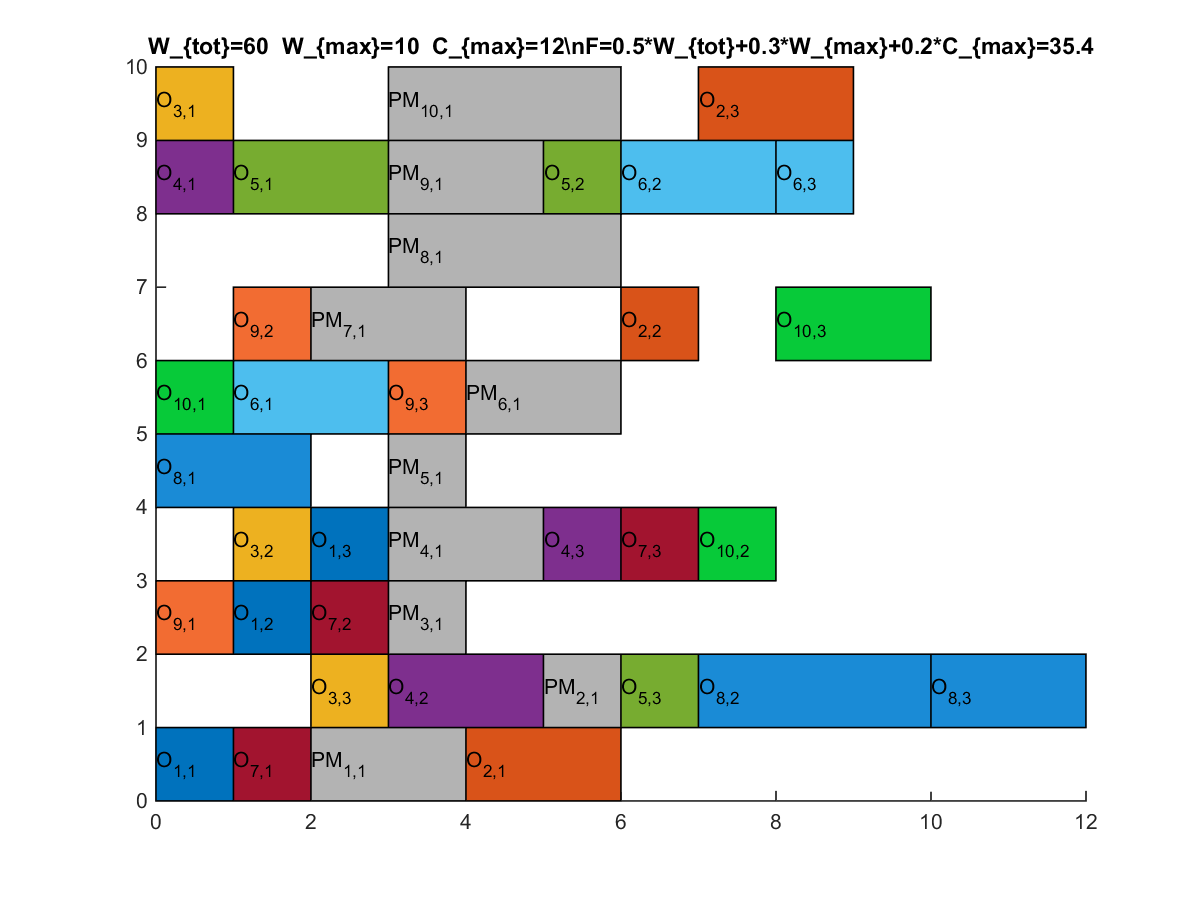
\includegraphics[width=0.8\textwidth]{img/results10x10_F050302.png}
  \caption{$10 \times 10$ $F(0.5;0.3;0.2)$ : $(W_t, W_{max}, C_{max}) = (60; 10; 12)$}
\end{figure}
\begin{figure}
  \centering
  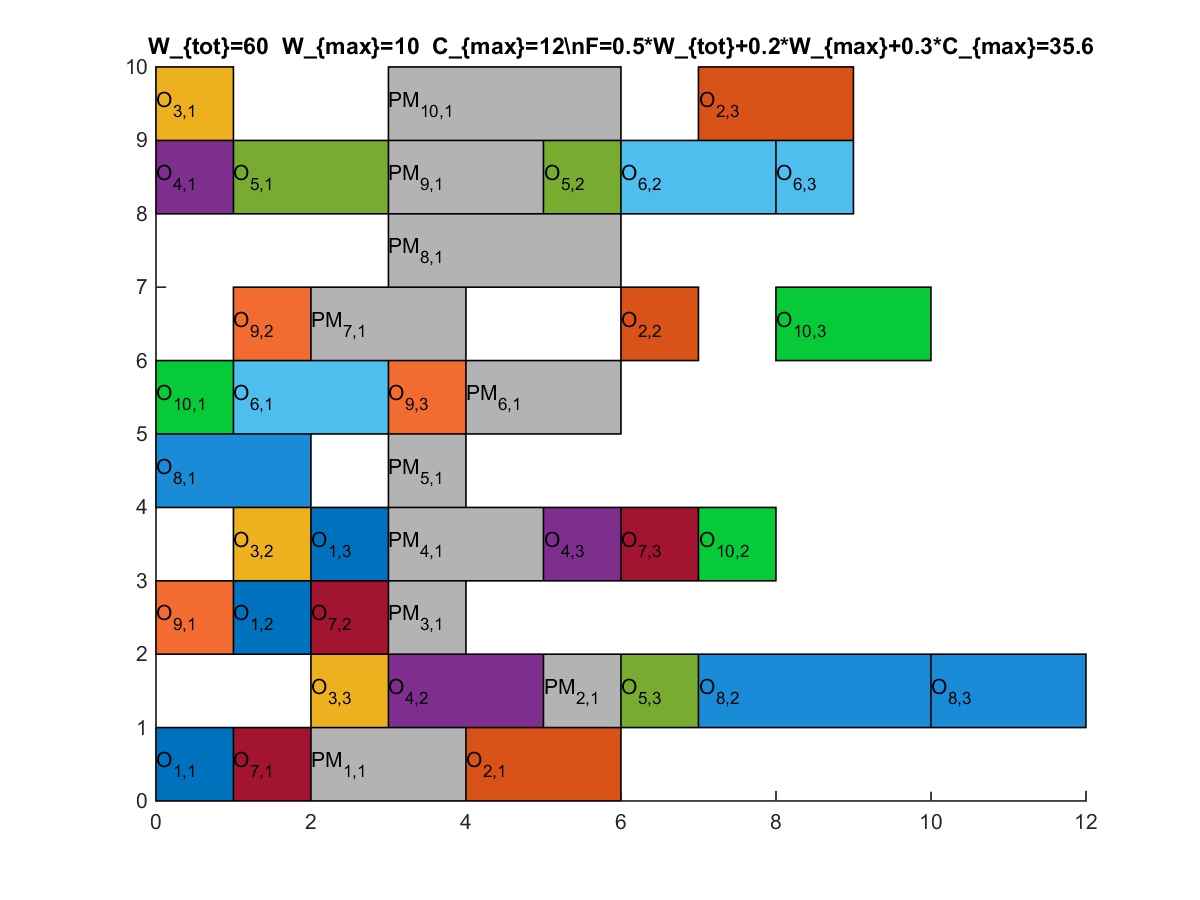
\includegraphics[width=0.8\textwidth]{img/results10x10_F050203.png}
  \caption{$10 \times 10$ $F(0.5;0.2;0.3)$ : $(W_t, W_{max}, C_{max}) = (60; 10; 12)$}
\end{figure}
\begin{figure}
  \centering
  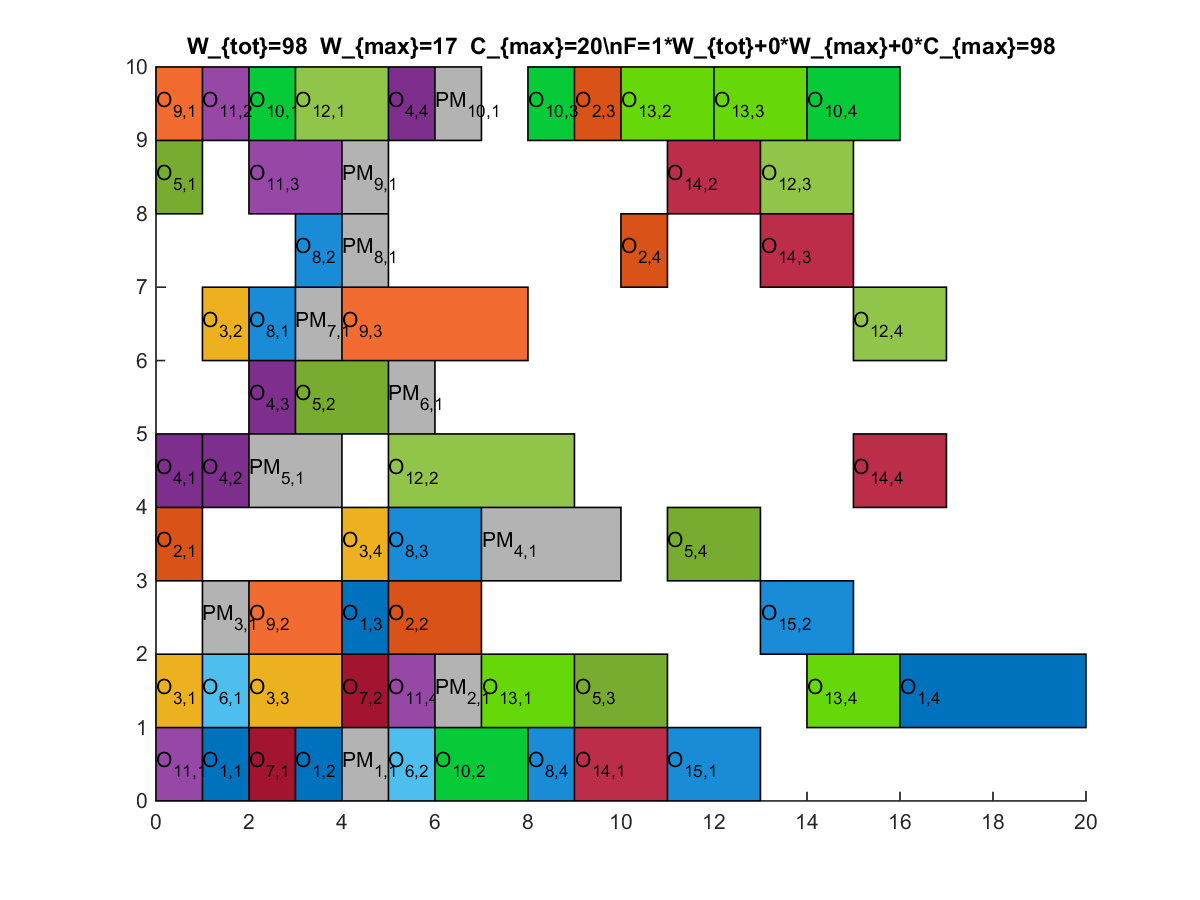
\includegraphics[width=0.8\textwidth]{img/results15x10_Wtot.png}
  \caption{$15 \times 10$ $W_{t}$ : $(W_t, W_{max}, C_{max}) = (98; 17; 20)$}
\end{figure}
\begin{figure}
  \centering
  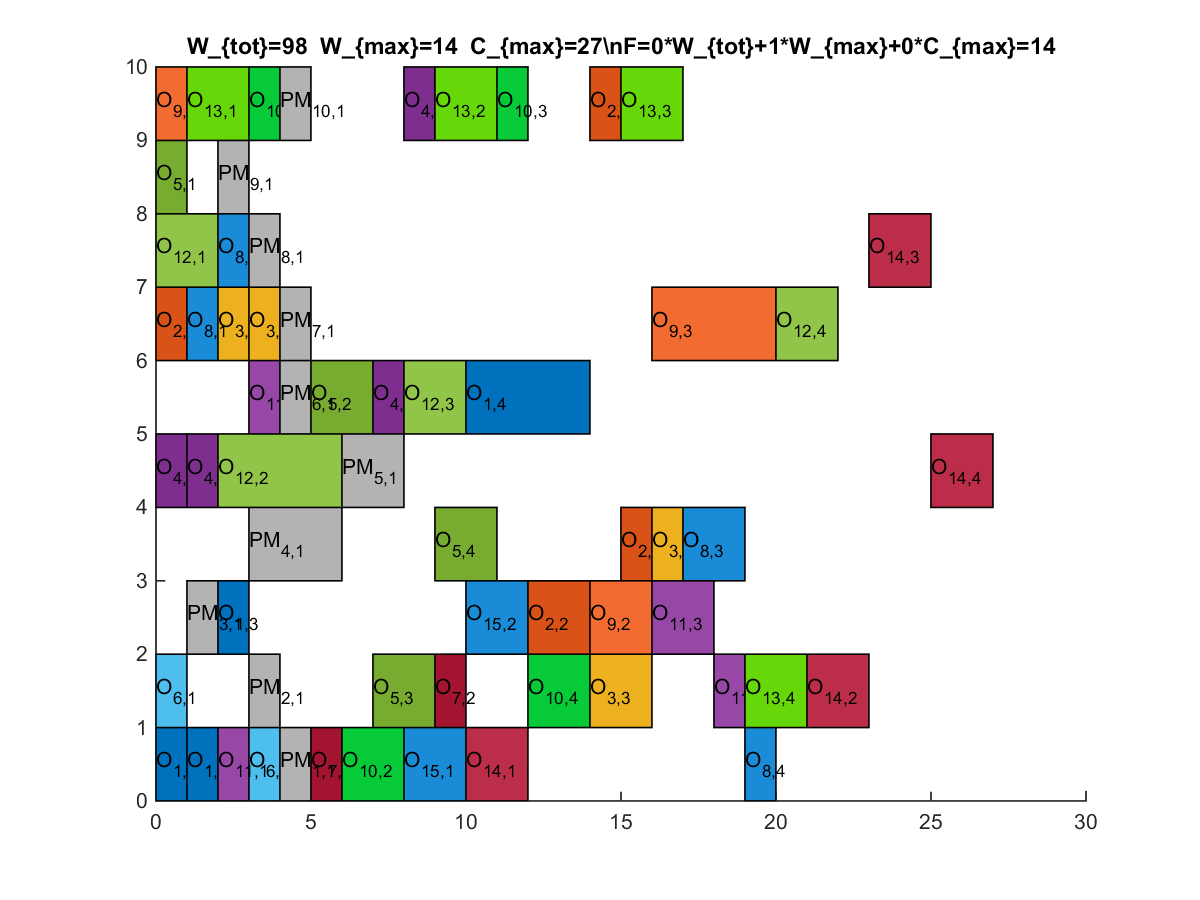
\includegraphics[width=0.8\textwidth]{img/results15x10_Wmax.png}
  \caption{$15 \times 10$ $W_{max}$ : $(W_t, W_{max}, C_{max}) = (98; 14; 27)$}
\end{figure}
\begin{figure}
  \centering
  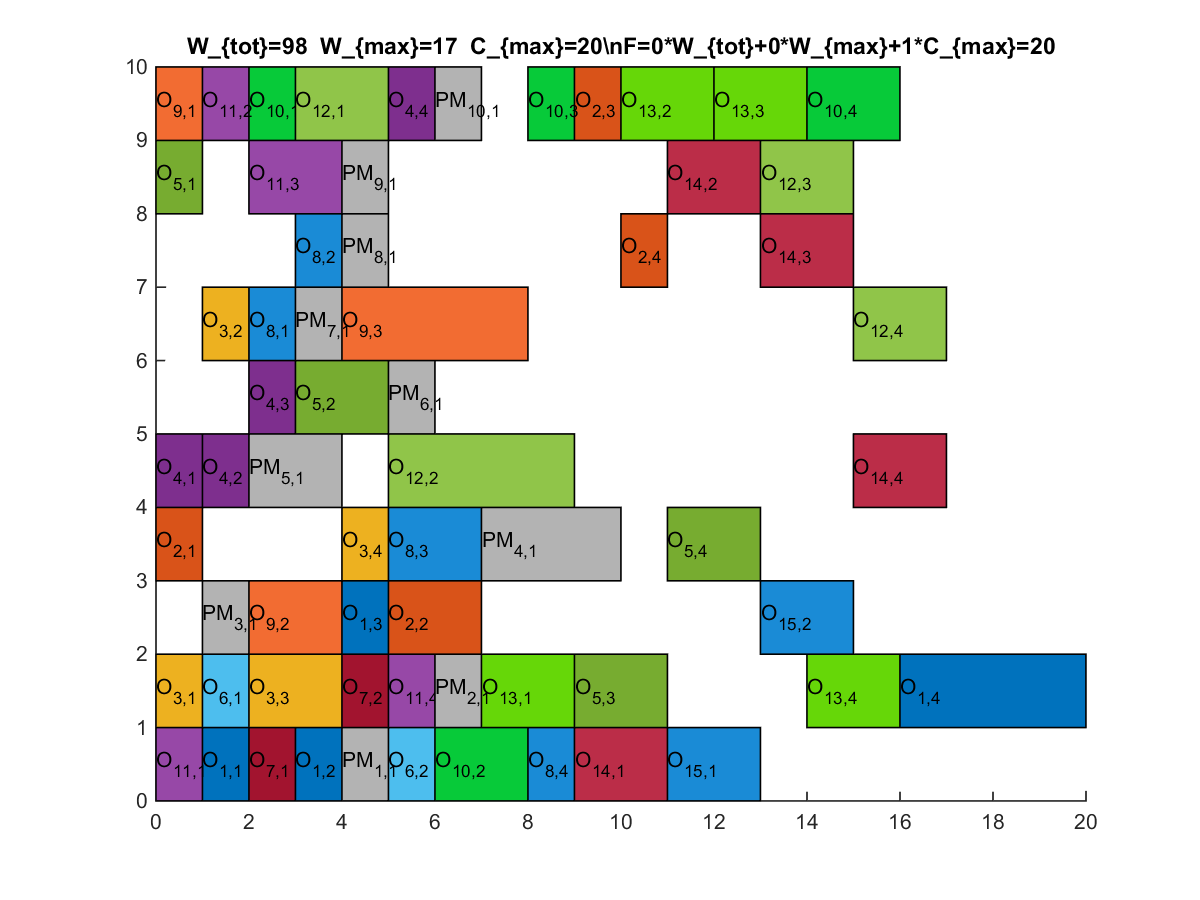
\includegraphics[width=0.8\textwidth]{img/results15x10_Cmax.png}
  \caption{$15 \times 10$ $C_{max}$ : $(W_t, W_{max}, C_{max}) = (106; 15; 19)$}
\end{figure}
\begin{figure}
  \centering
  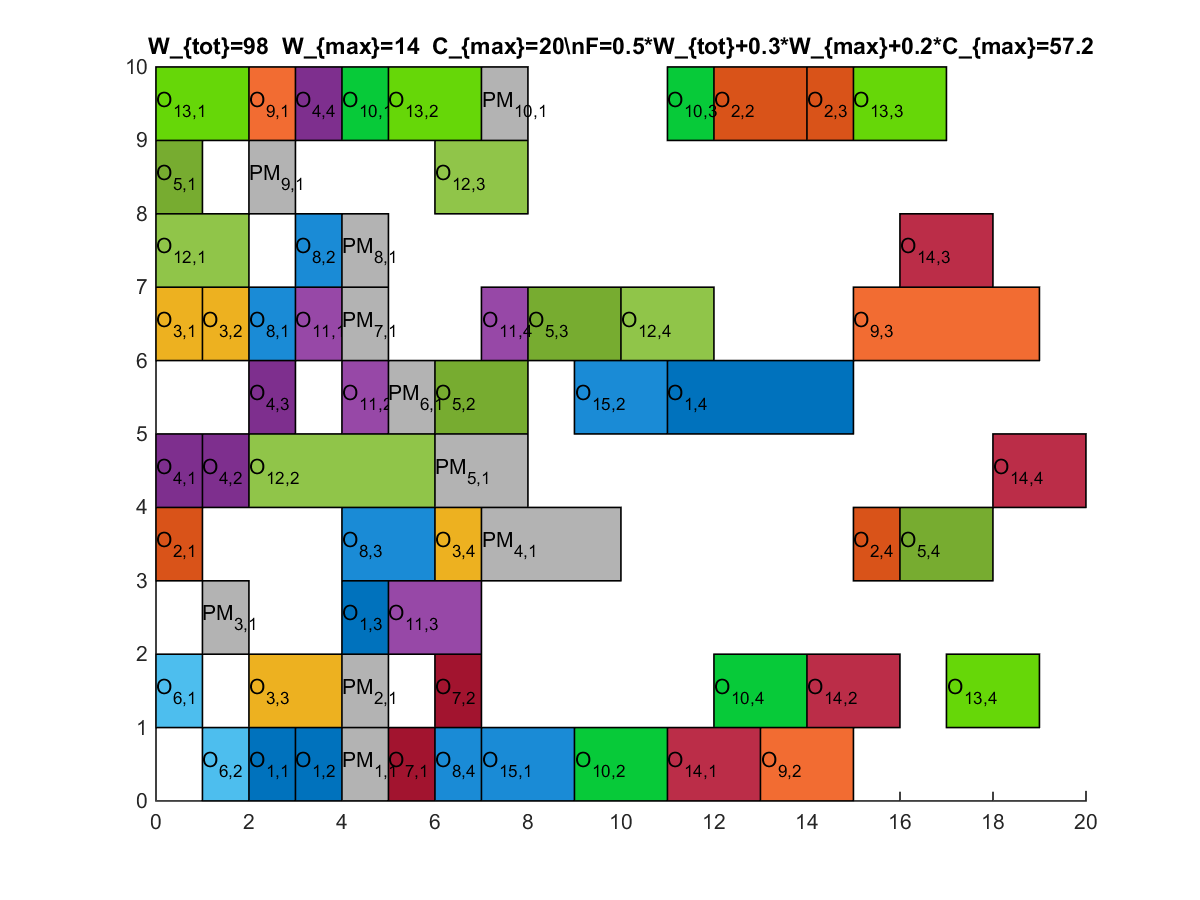
\includegraphics[width=0.8\textwidth]{img/results15x10_F050302.png}
  \caption{$15 \times 10$ $F(0.5;0.3;0.2)$ : $(W_t, W_{max}, C_{max}) = (98; 14; 20)$}
\end{figure}
\begin{figure}
  \centering
  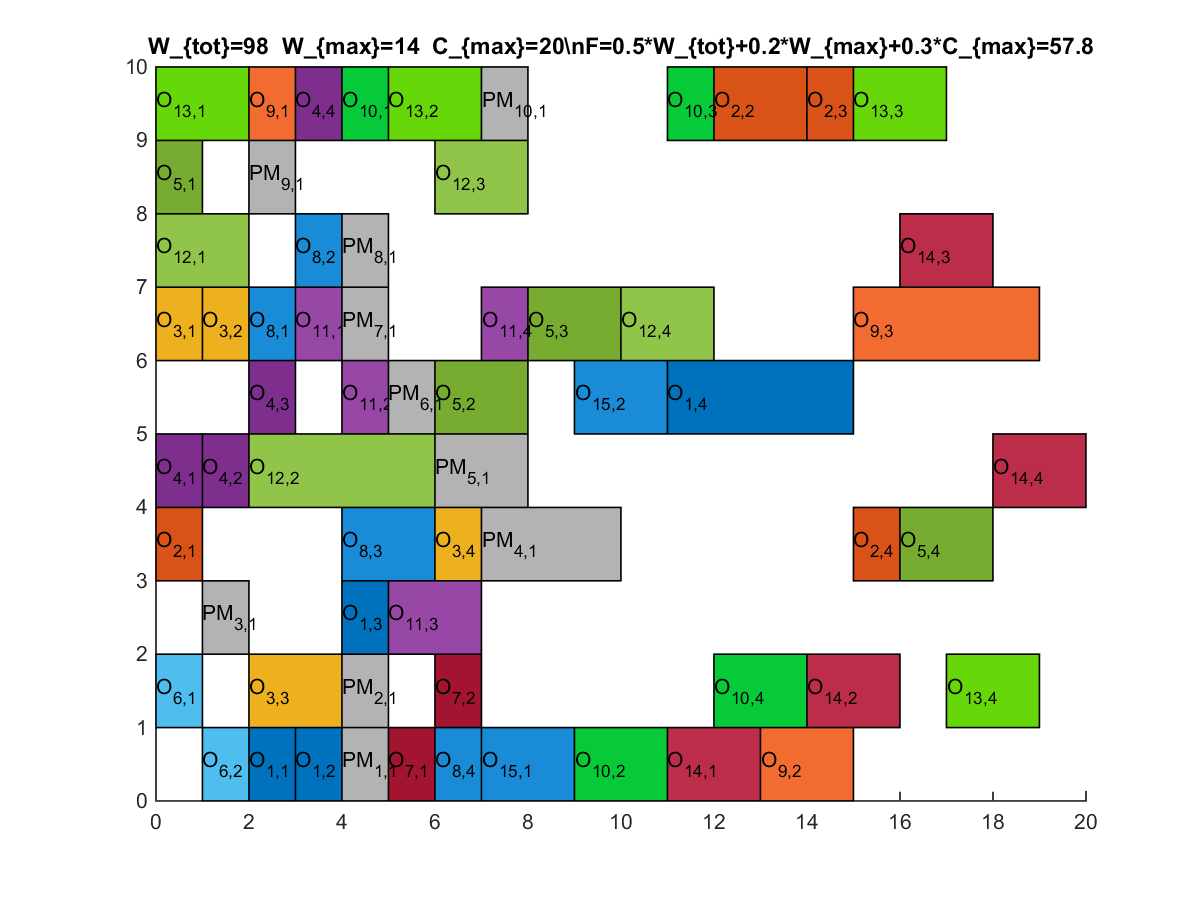
\includegraphics[width=0.8\textwidth]{img/results15x10_F050203.png}
  \caption{$15 \times 10$ $F(0.5;0.2;0.3)$ : $(W_t, W_{max}, C_{max}) = (98; 14; 20)$}
\end{figure}
\begin{figure}
  \centering
  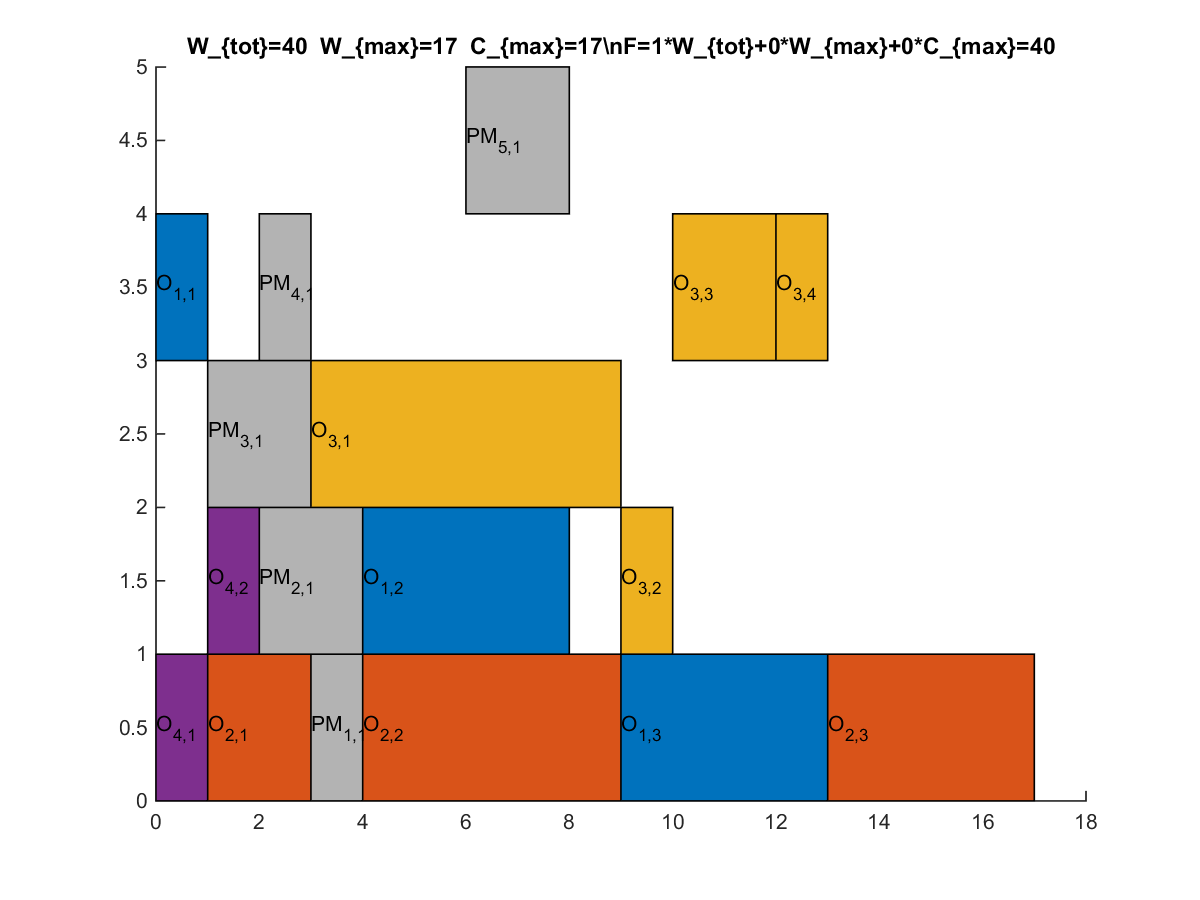
\includegraphics[width=0.8\textwidth]{img/results4x5_Wtot.png}
  \caption{$4 \times 5$ $W_{t}$ : $(W_t, W_{max}, C_{max}) = (40; 17; 17)$}
\end{figure}
\begin{figure}
  \centering
  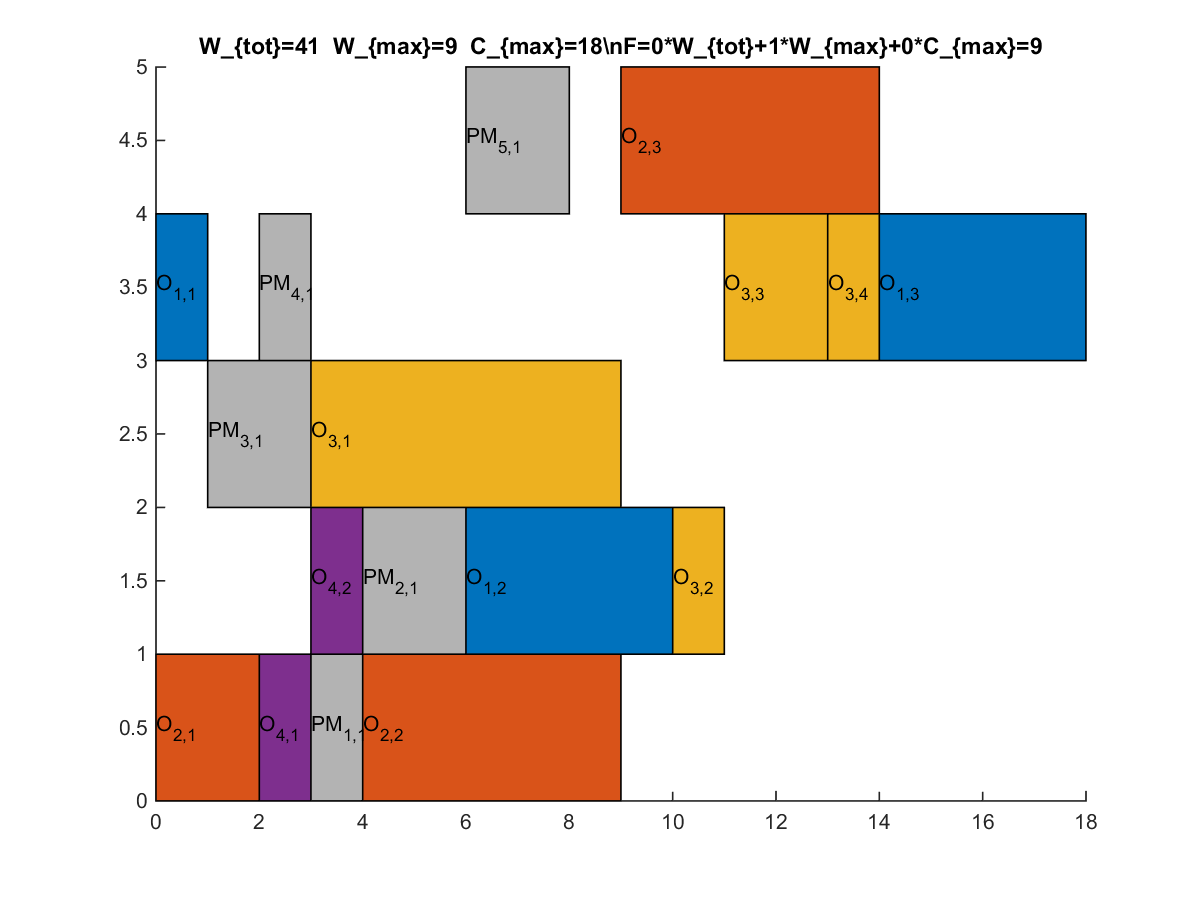
\includegraphics[width=0.8\textwidth]{img/results4x5_Wmax.png}
  \caption{$4 \times 5$ $W_{max}$ : $(W_t, W_{max}, C_{max}) = (41; 9; 18)$}
\end{figure}
\begin{figure}
  \centering
  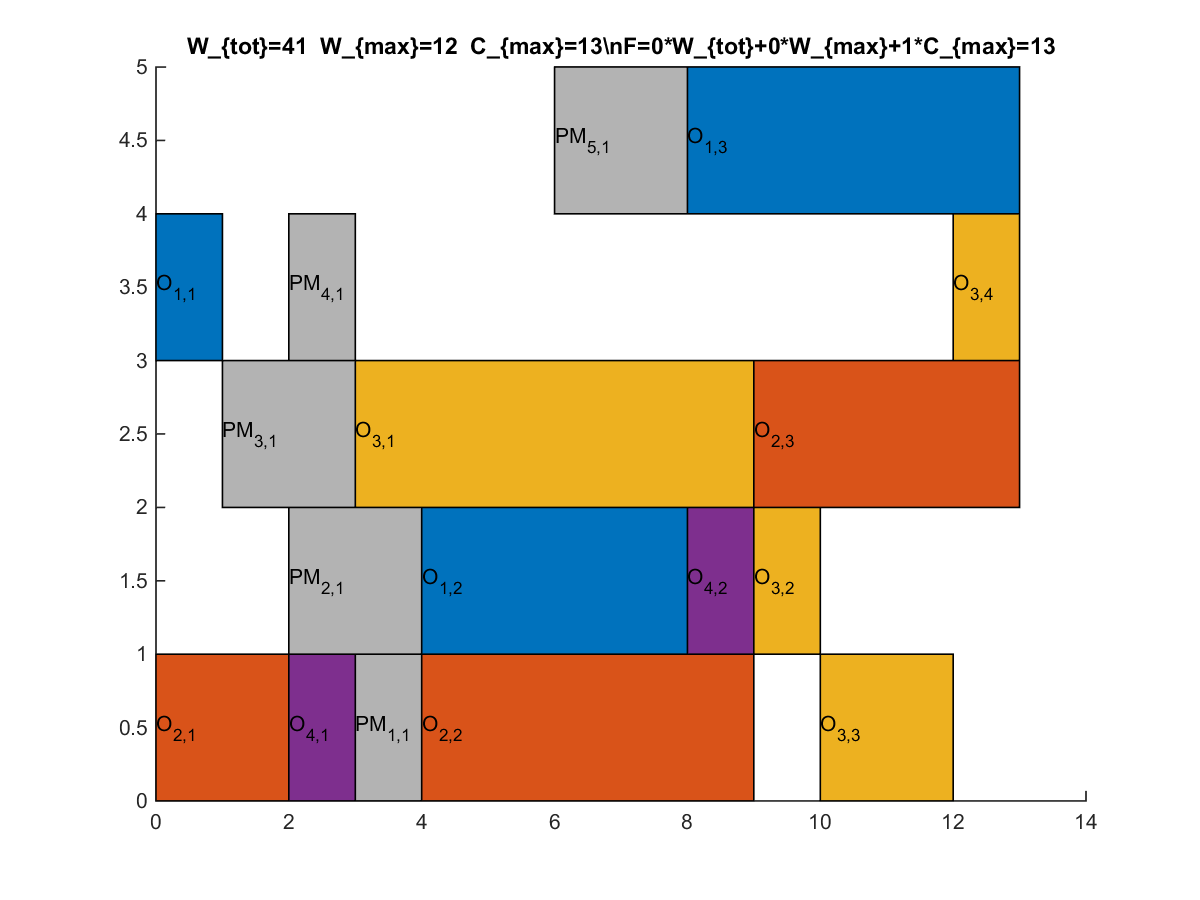
\includegraphics[width=0.8\textwidth]{img/results4x5_Cmax.png}
  \caption{$4 \times 5$ $C_{max}$ : $(W_t, W_{max}, C_{max}) = (41; 12; 12)$}
\end{figure}
\begin{figure}
  \centering
  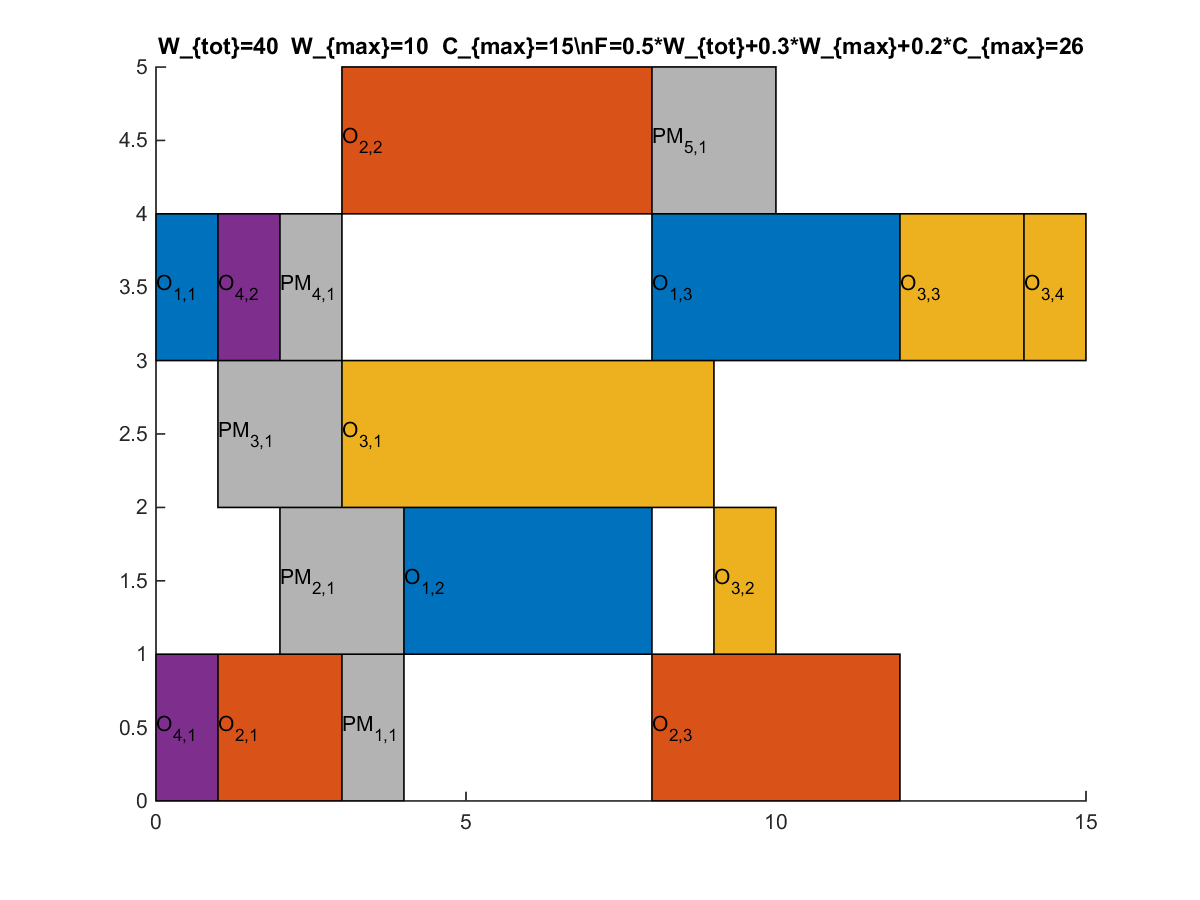
\includegraphics[width=0.8\textwidth]{img/results4x5_F050302.png}
  \caption{$4 \times 5$ $F(0.5;0.3;0.2)$ : $(W_t, W_{max}, C_{max}) = (40; 10; 13)$}
\end{figure}
\begin{figure}
  \centering
  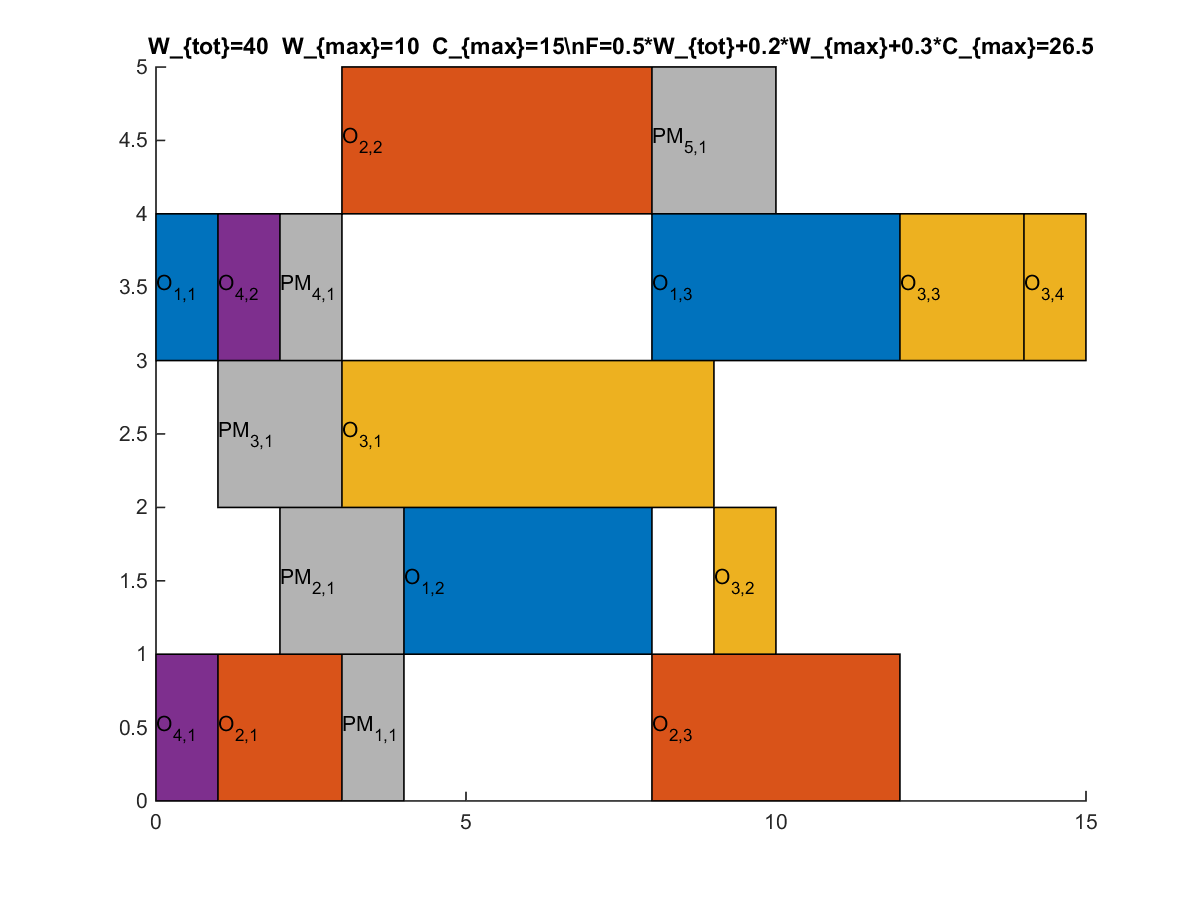
\includegraphics[width=0.8\textwidth]{img/results4x5_F050203.png}
  \caption{$4 \times 5$ $F(0.5;0.2;0.3)$ : $(W_t, W_{max}, C_{max}) = (40; 10; 13)$}
\end{figure}

\clearpage
\subsection{Visualisation des frontières de dominance de Pareto}
\label{annexe:visual_pareto}

\begin{figure}[!h]
  \centering
  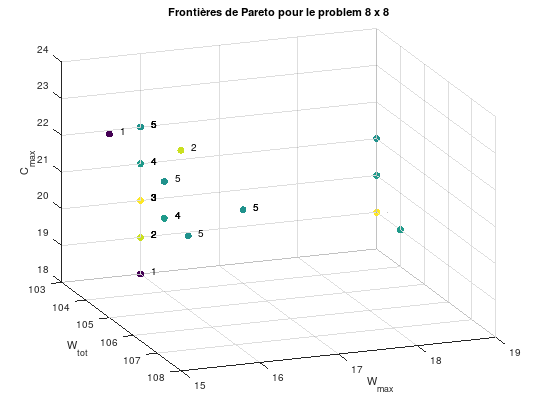
\includegraphics[width=0.8\textwidth]{img/results8x8_Pareto.png}
  \caption{5 Frontières de dominance de Pareto pour le problème 8x8}
\end{figure}
\begin{figure}
  \centering
  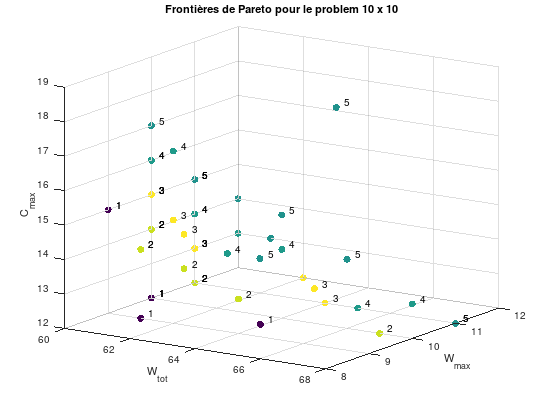
\includegraphics[width=0.8\textwidth]{img/results10x10_Pareto.png}
  \caption{5 Frontières de dominance de Pareto pour le problème 10x10}
\end{figure}
\begin{figure}
  \centering
  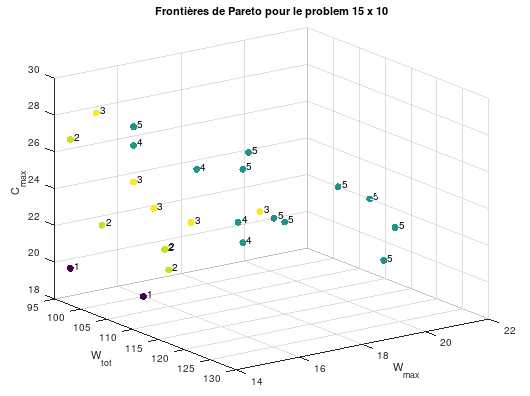
\includegraphics[width=0.8\textwidth]{img/results15x10_Pareto.png}
  \caption{5 Frontières de dominance de Pareto pour le problème 15x10}
\end{figure}
\begin{figure}
  \centering
  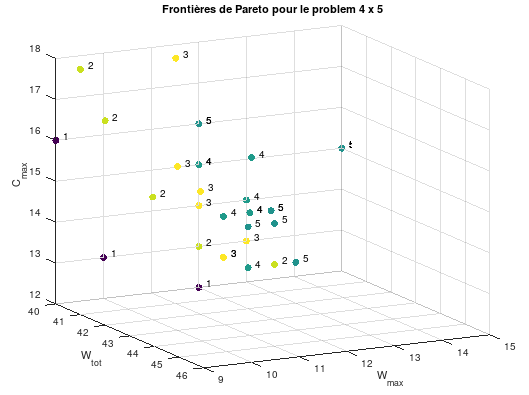
\includegraphics[width=0.8\textwidth]{img/results4x5_Pareto.png}
  \caption{5 Frontières de dominance de Pareto pour le problème 4x5}
\end{figure}

\clearpage

\begin{thebibliography}{1}
\addcontentsline{toc}{section}{Références}
\bibitem{GRASP}
   Rajkumar, Muthukannan \& Asokan, P \& Vamsikrishna, V. (2010),
   \emph{A GRASP algorithm for flexible job-shop scheduling with maintenance constraints},
    International Journal of Production Research - INT J PROD RES. 48. 6821-6836. 10.1080/00207540903308969. 

\bibitem{GA1}
	F. Pezzella, G. Morganti, G. Ciaschetti,
	\emph{A genetic algorithm for the Flexible Job-shop Scheduling Problem},
	Computers \& Operations Research,
	Volume 35, Issue 10,
	2008,
	Pages 3202-3212,
	ISSN 0305-0548,
	https://doi.org/10.1016/j.cor.2007.02.014.
	(http://www.sciencedirect.com/science/article/pii/S0305054807000524)
	
\bibitem{GA2}	
	T. S. Chan, F \& Wong, T. C. \& Chan, LY. (2006). 
	\emph{Flexible job-shop scheduling problem under resource constraints}, 
	International Journal of Production Research - INT J PROD RES. 44. 2071-2089. 10.1080/00207540500386012. 
\end{thebibliography}
\end{document}